\documentclass[a4paper,10pt]{article}

\usepackage[latin1]{inputenc}
\usepackage[T1]{fontenc}
\usepackage{amsmath}
\usepackage{amssymb}
\usepackage{enumerate}
\usepackage{multicol}
\usepackage{tikz, geometry}
\usepackage{xcolor, color, booktabs}	
\usepackage{graphicx}
\usepackage{grffile}
\usepackage{rotating}
\usepackage{wrapfig,lipsum}
\usepackage[font=scriptsize, position=top]{caption, subfig}
\graphicspath{{fig/}}
\usepackage{lscape}
\usepackage{alphalph}
\renewcommand\thesubfigure{\alphalph{\value{subfigure}}}

\title{Simulation results}
\author{}
\date{}

\newcommand\solidrule[1][0.5cm]{\rule[0.8ex]{#1}{1.5pt}}
\newcommand\dashedrule{\mbox{%
  \solidrule[1mm]\hspace{1mm}\solidrule[1mm]\hspace{1mm}\solidrule[1mm]}}
\newcommand\doubledashedrule{\mbox{%
  \solidrule[0.5mm]\hspace{0.5mm}\solidrule[0.5mm]\hspace{0.5mm}\solidrule[0.5mm]\hspace{0.5mm}\solidrule[0.5mm]\hspace{0.5mm}\solidrule[0.5mm]}}
\newcommand\dotdashdotrule{\mbox{%
  \solidrule[0.5mm]\hspace{1mm}\solidrule[2mm]\hspace{1mm}\solidrule[0.5mm]\hspace{0.5mm}}}

\setlength{\textheight}{11in}
\setlength{\textwidth}{6.5in}
\setlength{\topmargin}{-0.8in}
\setlength{\oddsidemargin}{-.3in}
\setlength{\evensidemargin}{-.3in}
\setlength{\headsep}{0in}

\definecolor{OliveGreen}{rgb}{0,0.6,0}
\newcommand{\bigbrk}{\vspace*{1.55in}}
\newcommand{\smallbrk}{\vspace*{.3in}}
\newcommand{\dif}{\mathrm{d}}%
\newcommand{\red}[1]{{\color{red}#1}}
\newcommand{\purple}[1]{{\color{purple}#1}}
\newcommand{\pink}[1]{{\color{pink}#1}}
\newcommand{\blue}[1]{{\color{blue}#1}}
\newcommand{\green}[1]{{\color{OliveGreen}#1}}
\newcommand{\brown}[1]{{\color{brown}#1}}
\newcommand{\lgray}[1]{{\color{lightgray}#1}}
\DeclareMathOperator{\logit}{logit}
\DeclareMathOperator{\Cov}{Cov}
\usetikzlibrary{calc}
\def\j{\mathbf j}

\begin{document}
\maketitle
\thispagestyle{empty} 
\pagestyle{empty}

\noindent
General model:
\begin{equation*}
\mu(t|Z) = f(t, \beta_0^\top Z)g(\gamma_0^\top Z),
\end{equation*}
where for fixed $x\in\mathbb{R}$,
$f(\cdot, x)$ is an unspecified density function on $[0, \tau]$, 
and $g(x)$ is unknown but monotone in $x$.
We assume $\|\beta_0\|=\|\gamma_0\|=1$.\newline

\textbf{Simulation settings used in the paper:} 
\begin{itemize}
\item $Z$ is generated from a multivariate truncated normal distribution 
satisfying $Z\sim N_2(0, I_2)$ and $\|Z\|\le1$.
\item Censoring time is an exponential distribution with mean $10\cdot(1 + |z_1|)$.
\item Recurrent event times are generated from Poisson process with rate functions:
\begin{description}
\item[M1:] $\mu(t|Z) = \mu_0(t) \exp(\gamma_0^\top Z)$
\begin{description}
\item[$\bullet$] $\mu_0(t) = \frac{2}{1 + t}$.
\item[$\bullet$] $\beta_0 = (\beta_1, \beta_2) = (0, 0)$, $\gamma_0 = (\gamma_1, \gamma_2) = (0.28, 0.96)$.
\end{description}
\item[M2:] $\mu(t|Z) = \mu_0(t) + \alpha_0^\top Z$
\begin{description}
\item[$\bullet$] $\mu_0(t) = e^{0.1t}$.
\item[$\bullet$] $\beta_0 = \gamma_0 = \alpha_0 = (0.6, 0.8)$.
\end{description}
\item[M3:] $\mu(t|Z) = \mu_0\{t\exp(\alpha_0^\top Z)\}$
\begin{description}
\item[$\bullet$] $\mu_0(t) = e^{-t}$.
\item[$\bullet$] $\beta_0 = \gamma_0 = \alpha_0 = (0.6, 0.8)$.
\end{description}
\item[M4:] $\mu(t|Z) = \mu_0\{t, \exp(\beta_0^\top Z)\}\exp(\gamma_0^\top Z)$
\begin{description}
\item[$\bullet$] $\mu_0(t, x) = \frac{t\cdot(1 - t)^{1+x}}{B(2, 1+x)}$
\item[$\bullet$] $\beta_0 = (0.6, 0.8)$, $\gamma_0 = (0.28, 0.96)$
\end{description}
\end{description}
\item Set $\tau = 10$ for \textbf{M1, M2, M3} and $\tau = 1$ for \textbf{M4}.
\item \textbf{M1-ind} solves $\gamma_0$ under shape-independence.
\end{itemize}

\begin{table}[ht]
\centering
%\renewcommand\tabcolsep{2pt}
\caption{Point estimator (PE), empirical standard error (ESE) and asymptotic standard error (ASE) for \textbf{M1}--\textbf{M4} with 1000 replications.}
\begin{tabular}{r rrr rrr rrr rrr}
\toprule
& \multicolumn{3}{c}{$n=50$} & \multicolumn{3}{c}{$n=100$} & \multicolumn{3}{c}{$n=200$} & \multicolumn{3}{c}{$n=500$}\\
\cmidrule(l){2-4}\cmidrule(l){5-7}\cmidrule(l){8-10}\cmidrule(l){11-13}
& PE & ESE & ASE & PE & ESE & ASE & PE & ESE & ASE & PE & ESE & ASE \\
\midrule
& \multicolumn{12}{c}{Scenario \textbf{M1}; without assuming shape-independent.}\\
[1ex]
$\beta_1$ & 0.302 & 0.626 & 0.488 & 0.196 & 0.662 & 0.502 & 0.151 & 0.667 & 0.515 & 0.102 & 0.679 & 0.520 \\ 
$\beta_2$ & 0.300 & 0.654 & 0.493 & 0.276 & 0.670 & 0.515 & 0.264 & 0.681 & 0.526 & 0.152 & 0.712 & 0.539 \\ 
$\gamma_1$ & 0.273 & 0.114 & 0.133 & 0.276 & 0.082 & 0.087 & 0.274 & 0.076 & 0.060 & 0.279 & 0.037 & 0.036 \\ 
$\gamma_2$ & 0.955 & 0.032 & 0.038 & 0.957 & 0.025 & 0.025 & 0.958 & 0.029 & 0.018 & 0.960 & 0.010 & 0.011 \\ 
[1ex]
& \multicolumn{12}{c}{Scenario \textbf{M1}; assuming shape-independent.}\\
[1ex]
$\gamma_1$ & 0.264 & 0.118 & 0.141 & 0.272 & 0.077 & 0.089 & 0.276 & 0.054 & 0.059 & 0.275 & 0.033 & 0.035 \\ 
$\gamma_2$ & 0.957 & 0.031 & 0.038 & 0.959 & 0.021 & 0.023 & 0.960 & 0.015 & 0.016 & 0.961 & 0.009 & 0.010 \\ 
[1ex]
& \multicolumn{12}{c}{Scenario \textbf{M2}.}\\
[1ex]
$\beta_1$ & $-$0.194 & 0.655 & 0.566 & $-$0.435 & 0.456 & 0.522 & $-$0.592 & 0.197 & 0.379 & $-$0.597 & 0.073 & 0.099 \\ 
$\beta_2$ & $-$0.296 & 0.669 & 0.567 & $-$0.606 & 0.486 & 0.520 & $-$0.743 & 0.245 & 0.396 & $-$0.797 & 0.054 & 0.094 \\ 
$\gamma_1$ & 0.591 & 0.116 & 0.132 & 0.599 & 0.086 & 0.092 & 0.593 & 0.076 & 0.067 & 0.597 & 0.051 & 0.047 \\ 
$\gamma_2$ & 0.792 & 0.099 & 0.109 & 0.793 & 0.068 & 0.078 & 0.800 & 0.052 & 0.053 & 0.797 & 0.085 & 0.036 \\ 
[1ex]
& \multicolumn{12}{c}{Scenario \textbf{M3}.}\\
[1ex]
$\beta_1$ & $-$0.080 & 0.670 & 0.576 & $-$0.376 & 0.513 & 0.545 & $-$0.584 & 0.172 & 0.407 & $-$0.602 & 0.057 & 0.088 \\ 
$\beta_2$ & $-$0.304 & 0.673 & 0.570 & $-$0.594 & 0.492 & 0.528 & $-$0.775 & 0.170 & 0.388 & $-$0.795 & 0.042 & 0.083 \\ 
$\gamma_1$ & $-$0.415 & 0.493 & 0.531 & $-$0.561 & 0.220 & 0.397 & $-$0.594 & 0.083 & 0.150 & $-$0.599 & 0.047 & 0.050 \\ 
$\gamma_2$ & $-$0.567 & 0.514 & 0.522 & $-$0.765 & 0.225 & 0.371 & $-$0.798 & 0.055 & 0.140 & $-$0.797 & 0.056 & 0.039 \\ 
[1ex]
& \multicolumn{12}{c}{Scenario \textbf{M4}.}\\
[1ex]
$\beta_1$ & $-$0.070 & 0.672 & 0.569 & $-$0.312 & 0.548 & 0.547 & $-$0.556 & 0.269 & 0.445 & $-$0.597 & 0.063 & 0.132 \\ 
$\beta_2$ & $-$0.271 & 0.686 & 0.570 & $-$0.534 & 0.564 & 0.533 & $-$0.743 & 0.259 & 0.419 & $-$0.798 & 0.047 & 0.125 \\ 
$\gamma_1$ & 0.251 & 0.217 & 0.231 & 0.266 & 0.142 & 0.153 & 0.274 & 0.094 & 0.102 & 0.280 & 0.059 & 0.062 \\ 
$\gamma_2$ & 0.941 & 0.068 & 0.078 & 0.953 & 0.041 & 0.042 & 0.957 & 0.025 & 0.029 & 0.958 & 0.017 & 0.019 \\ 
\bottomrule
\end{tabular}
\end{table}

\begin{table}[ht]
\centering
\caption{Summary of rejection proportions based on the simulation scenarios \textbf{M1}--\textbf{M4}.
The rejection proportions are computed based on $n=50, 100, 200, 500$ observations with 1000 replications at $\alpha = 0.05$.
The resampling size is 200. 
}
\begin{tabular}{rrrrr}
\toprule
& \multicolumn{4}{c}{$n$}\\
\cmidrule(l){2-5}
& 50 & 100 & 200 & 500 \\
\midrule
\textbf{M1} & 0.031 & 0.037 & 0.046 & 0.052 \\ 
\textbf{M2} & 0.281 & 0.700 & 0.960 & 1.000 \\ 
\textbf{M3} & 0.382 & 0.831 & 0.996 & 1.000 \\ 
\textbf{M4} & 0.287 & 0.686 & 0.963 & 1.000 \\ 
\bottomrule
\end{tabular}
\end{table}

\newpage
\paragraph{Rank estimating equation with induced smoothing}
The rank estimating equation 
\begin{equation*}
\label{E1}
U_1(\beta) = \frac{1}{n(n-1)}\sum_{i\neq j} I(\beta^\intercal Z_i >  \beta^\intercal Z_j) \int_{0}^{C_{ij}} \int_{0}^{C_{ij}} I( u>t)dN_i(u)dN_j(t),
\end{equation*}
is sensitive to initial value; local maximums are often detected instead of the global maximum.

The motivation of the induced smoothing technique is to overcome computational difficulty caused by non-smooth estimating equations. 
The basic idea is to replace the estimating equation $U_1(\beta)$ with a smooth version
$E(\beta+ \Gamma Z)$, 
where $Z$ is a $p$-dimensional standard normal random vector, $\Gamma^\top\Gamma = \Sigma$ is the 
a working covariance matrix of $\hat\beta_n$, and the expectation is taken with respect to $Z$.
The smoothed version of $U_1(\beta)$ is then
\begin{equation}
\label{smooth}
\tilde U_1(\beta) = \frac{1}{n(n-1)}\sum_{i\neq j} \Phi\left(\frac{\beta^\intercal Z_i -  \beta^\intercal Z_j}{r_{ij}}\right) \int_{0}^{C_{ij}} \int_{0}^{C_{ij}} I( u>t)dN_i(u)dN_j(t),
\end{equation}
where $r_{ij}^2 = (X_i - X_j)^\top\Gamma_n(X_i - X_j)$.
In my other papers, we tried different choices of $\Gamma$ but all yields similar results, 
so I usually set $\Gamma$ to be the identity matrix. 

In Figure~\ref{comp}, I plotted the \textbf{negative} $U_1(\cdot)$ and $\tilde U_1(\cdot)$ values against $\theta$ for one simulated data set with $n = 100$ from scenario M2. (so we are looking to find the global minimum here). 
There are many local minimums for the unsmoothed estimating equation, causing the \texttt{optim} and \texttt{spg} to converge to one of the local minimums. However, we don't have such problem with the smoothed version. Simulation results that shows the $\beta$ estimates by optimizing the smoothed estimating equation based on 200 replications is presented in Table 3. 

\begin{center}
\begin{figure}
\caption{Comparison between $U_1(\beta)$ and $\tilde U_1(\beta)$.}
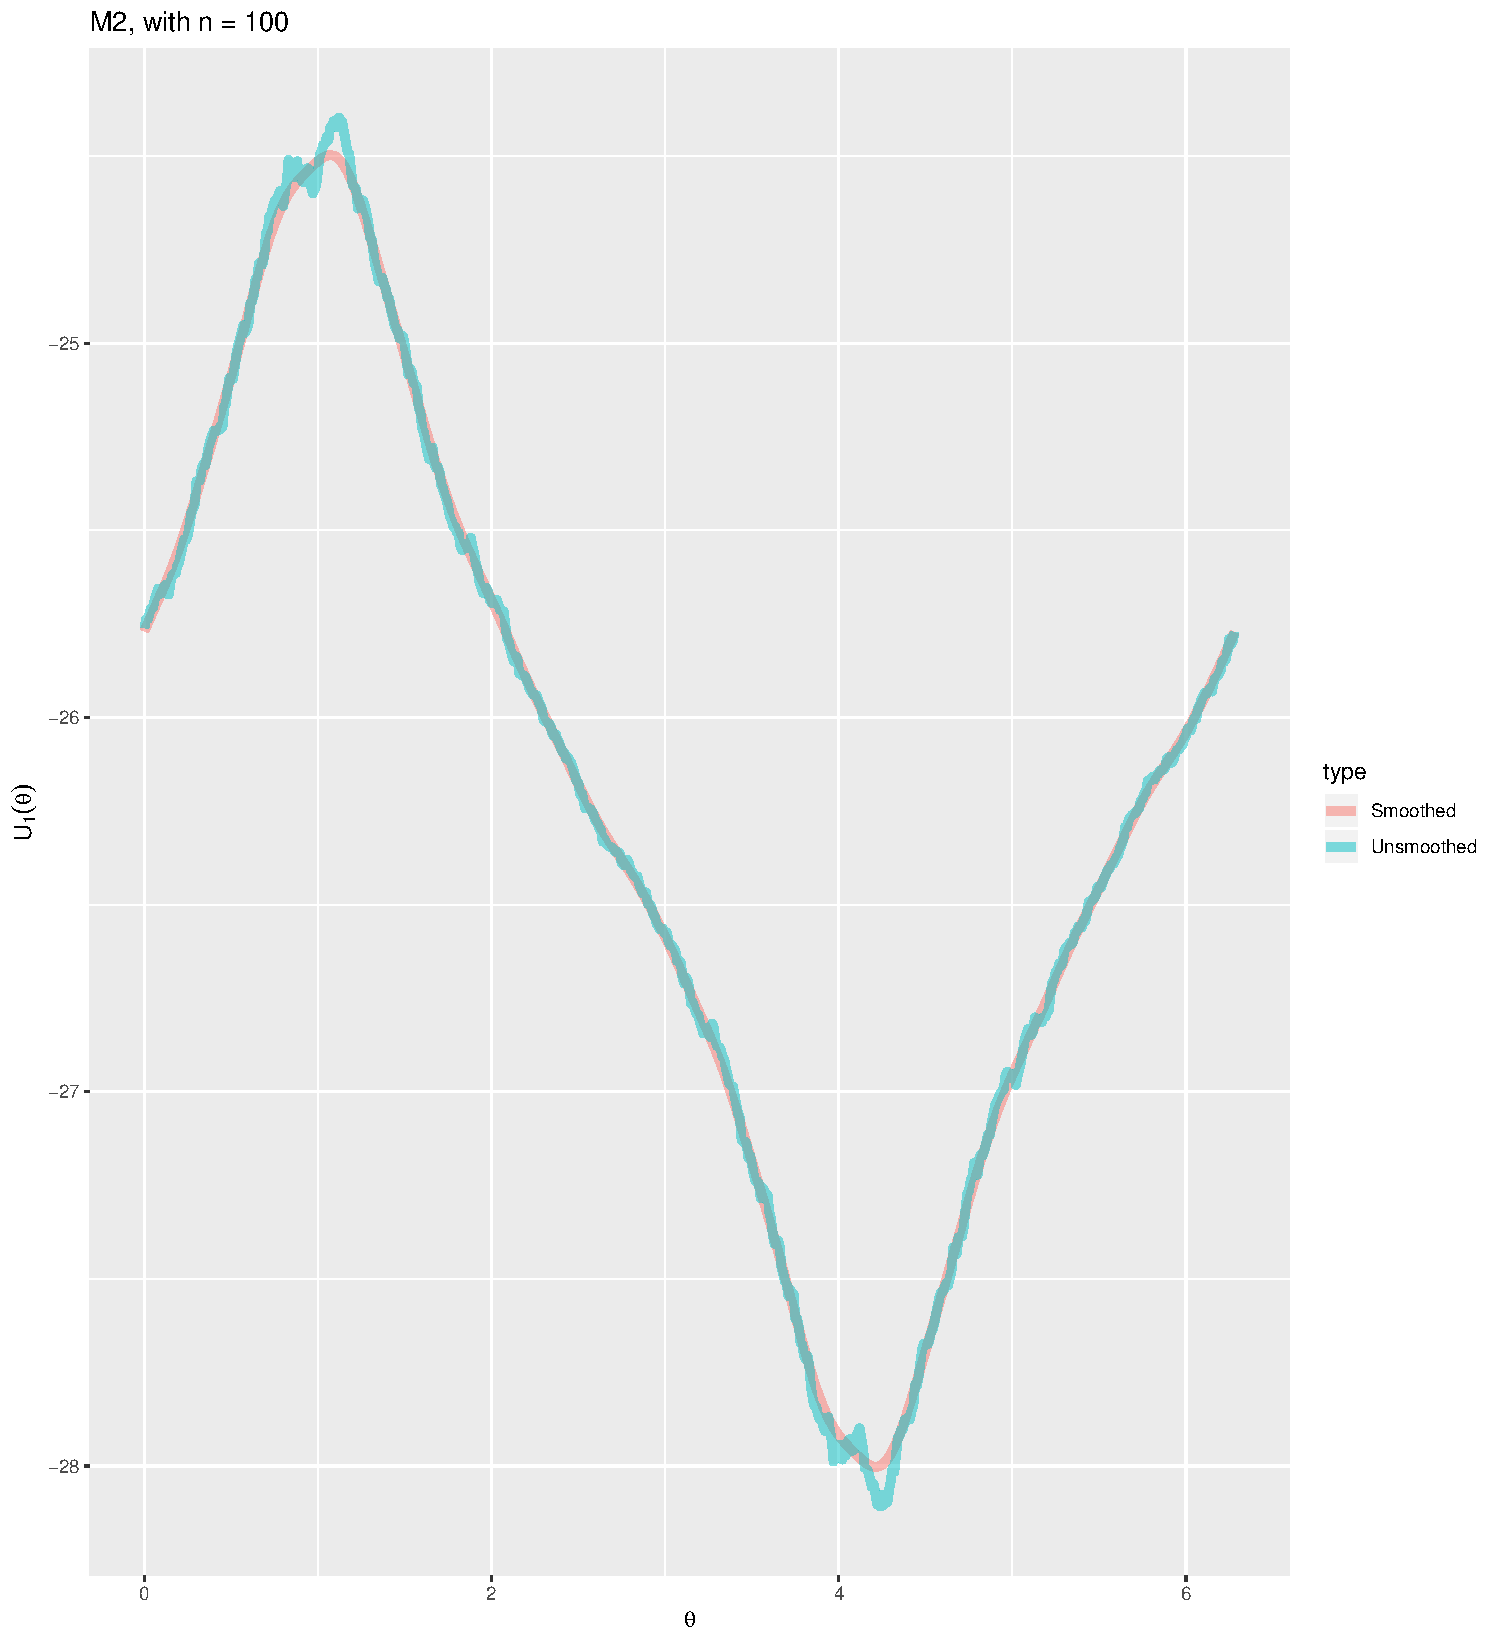
\includegraphics[scale = .6]{rank.pdf}\label{comp}
\end{figure}
\end{center}

\begin{table}[ht]
\centering
\caption{Simulation results based on induced smoothing equation~\eqref{smooth}. 
With 200 replications. 
All replications converged to global maximum (verified with an exhaust grid search).
$\Gamma$ is set to be the identity matrix.}
\begin{tabular}{r rrrrrr}
\toprule
& \multicolumn{2}{c}{$n=100$} & \multicolumn{2}{c}{$n=200$} & \multicolumn{2}{c}{$n=500$} \\
\cmidrule(l){2-3}\cmidrule(l){4-5}\cmidrule(l){6-7}
& PE & ESE& PE & ESE& PE & ESE\\
\midrule
& \multicolumn{6}{c}{Scenario \textbf{M2}}\\
$\beta_1$ &  -0.582 & 0.184 & -0.599 & 0.125 & -0.593 & 0.075 \\ 
$\beta_2$ &  -0.764 & 0.209 & -0.784 & 0.104 & -0.799 & 0.055 \\ 
$\gamma_1$ &  0.588 & 0.118 & 0.599 & 0.057 & 0.593 & 0.033 \\ 
$\gamma_2$ &  0.786 & 0.150 & 0.797 & 0.042 & 0.804 & 0.024 \\ 
& \multicolumn{6}{c}{Scenario \textbf{M3}}\\
$\beta_1$ &   -0.601 & 0.161 & -0.591 & 0.096 & -0.601 & 0.052 \\ 
$\beta_2$ &   -0.774 & 0.124 & -0.797 & 0.075 & -0.797 & 0.040 \\ 
$\gamma_1$ &   -0.602 & 0.120 & -0.595 & 0.066 & -0.600 & 0.044 \\ 
$\gamma_2$ &   -0.782 & 0.113 & -0.799 & 0.051 & -0.798 & 0.033 \\
\bottomrule
\end{tabular}
\end{table}

\end{document}